\documentclass[11pt,a4paper]{article}
\usepackage[top=1.00in, bottom=1.0in, left=1in, right=1in]{geometry}
\usepackage{graphicx}
\usepackage{sectsty,setspace,natbib,wasysym} 
\usepackage{natbib}
\usepackage{parskip}

\begin{document}
\bibliographystyle{/Users/Lizzie/Documents/EndnoteRelated/Bibtex/styles/naturemag}
\hspace{-5ex} \includegraphics[width=0.4\textwidth]{/Users/Lizzie/Documents/Professional/images/letterhead/ubc/Faculty of forestry 2026short.png}
\pagenumbering{gobble}

\vspace{2ex}
\begin{small}
\noindent 2424 Main Mall \\
\noindent Vancouver, BC Canada V6T 1Z4\\
\noindent Ph: 604.827.5246\\
\end{small}
\vspace{2ex}\\
\pagenumbering{gobble}
\noindent Dear Dr. Way:

Please consider our paper, entitled `The problem and promise of modeling plant leafout under warmer winters,' as a perspective for  \emph{Global Change Biology}. 

\emph{What scientific question is addressed in this manuscript?} % 43

Why do current models of leafout timing with climate change make wildly different predictions for the same system and temperature regime? How can simple models from the 1970s still be  equally predictive as newer models, despite apparent progress over the last decades?  
% We focus chilling, a concept with major implications for many fruit crops and how well forests can continue to sequester carbon with climate change. We address why current models predict wildly different leafout times for the same system and temperature regime, with little progress over the last decades.

\emph{What is/are the key finding(s) that answer this question?} % 43

We argue progress has stalled because we do not understand how winter temperatures affect leafout. Models today estimate the effect of winter temperatures via an unobserved process called chilling. This has produced fundamental problems that the field has struggled to admit or address. %  through the concept of chilling. We highlight fundamental problems with chilling---an unobserved process---that impact all models of plant leafout today. 
% These include the reality that chilling is an unobserved process, which may lead to current highly uncertain and variable forecasts. We suggest a path towards more mechanistic models that build on and help design experimental results. 

\emph{Why is this work important and timely?} % 44

Interest in chilling for forecasting the effects of climate change has led to myriad new models, but few insights. In this perspective we argue that major advances through molecular and other new approaches will be slow without a reckoning with the concept of chilling. 

\emph{Describe how your paper fits within the scope of GCB.} % 50
% Global Change Biology is an environmental change journal dedicated to shaping the future and solving the world's most challenging problems by tackling sustainability, climate change and environmental protection, food and water safety and provision, as well as global health.

We bring a cross-disciplinary and solutions-focused perspective on chilling, a concept critical to predicting and mitigating impacts of climate change. We bridge across ecological forecasting, molecular biology, forest tree and crop modelers to highlight the problems that may limit the potential for rapid progress, and show how to fix them. 

\emph{What biological AND global change aspects does it address?} % 45

Chilling is a fundamental concept in plant biology with major implications for many fruit crops and how well forests can continue to sequester carbon with climate change. An improved understanding of chilling is integral to managing agricultural, horticultural, and forest systems with continued climate change. % 

\emph{What are the three most recently published papers that are relevant to this manuscript?} 

Baumgarten, F., Zohner, C.M., Gessler, A. and Vitasse, Y. (2021), Chilled to be forced: the best dose to wake up buds from winter dormancy. \emph{New Phytologist} 230: 1366-1377. 

Ettinger, A.K., Chamberlain, C.J., Morales-Castilla, I., Buonaiuto, D.M., Flynn, D.F.B., Savas, T., Samaha, J.A. \& Wolkovich, E.M. (2020) Winter temperatures predominate in spring phenological responses to warming. \emph{Nature Climate Change} 10, 1137–U119.\\

% Pan, W., Li, J., Du, Y., Zhao, Y., Xin, Y., Wang, S., Liu, C., Lin, Z., Fang, S., Yang, Y. et al. (2023) Epigenetic silencing of callose synthase by VIL1 promotes bud-growth transition in lily bulbs. Nature Plants 9, 1451–1467.\\

Zhao, Y., Antoniou-Kourounioti, R.L., Calder, G., Dean, C. \& Howard, M. (2020) Temperature- dependent growth contributes to long-term cold sensing. \emph{Nature} 583, 825–829.

\emph{Provide the name and institutional email addresses of 5 potential reviewers.}\\
Guillaume Charrier: guillaume.charrier@inrae.fr\\
Andrew Richardson: Andrew.Richardson@nau.edu\\
Josh M Gray: josh\_gray@ncsu.edu\\
Christy Rollinson: crollinson@mortonarb.org\\
Lynsay Spafford: lspaffor@stfx.ca\\
Mark Freidl: friedl@bu.edu

I and my co-authors believe this perspective would be of interest to readers \emph{Global Change Biology} and look forward to hearing from you. If have additional questions, please let me know. 
\vspace{1.5ex}\\
Sincerely,\\

\includegraphics[scale=1]{/Users/Lizzie/Documents/Professional/Vitas/Signatures/SignatureLizzieSm.png} \\

\noindent Elizabeth M Wolkovich\\
Associate Professor of Forest \& Conservation Sciences\\ 

% This paper: https://onlinelibrary.wiley.com/doi/full/10.1111/geb.13932

\end{document}


The piece focuses on chilling---the concept of cool temperatures required to break dormancy---with a focus on woody plant flowering and leafing, where the concept has major implications for many fruit crops and how well forests can continue to sequester carbon with climate change \citep{keenan2014net,ipcc2022}. This is also where forecasts of shifts in chilling with climate change yield almost endless possibilities: current models predict wildly different leafout or flowering times for the same study system and temperature regime \citep[][]{basler2016evaluating,hufkens2018integrated}. Interest in chilling for forecasting the effects of climate change has led to myriad new models, but few insights. 

In this perspective we argue that major advances through molecular approaches \citep[e.g.,][]{zhu2021cold,azeez2021early,pan2023epigenetic,cai2024molecular} will be slow without a  reckoning with the concept of chilling. We highlight fundamental problems with the concept, including the reality that it is an unobserved process, representing the transition between two latent states. The result of this in models of chilling today is hidden assumptions and obscured work-arounds leading to highly uncertain and variable forecasts. We show how new molecular advances may rule out certain common models, and suggest a path towards more mechanistic models that build on and help design experimental results. We close by and asking whether the concept of `chilling' may soon be unnecessary for scientific progress. 

Our perspective aims to bridge across the often siloed fields that work on chilling---molecular biologists, forest tree and crop modelers, and those focused on forecasting with climate change---to uncover the problems that may limit the potential for rapid progress through new experimental work. As such we leverage existing data from different fields to show how common some of the unspoken problems with current approaches are. I include below a potential abstract and several potential figures. 

If you think this article could be of interest to readers of \emph{Global Change Biology} or have additional questions, please let me know. 
\vspace{1.5ex}\\
Sincerely,\\

\includegraphics[scale=1]{/Users/Lizzie/Documents/Professional/Vitas/Signatures/SignatureLizzieSm.png} \\

\noindent Elizabeth M Wolkovich\\
Professor of Forest \& Conservation Sciences\\ 

{\bf Abstract:} How warmer winters affect plant budburst has major implications for carbon storage and ecosystem stability. Recent evidence that the advance of spring leafout has slowed with anthropogenic climate change has reignited a decades-old debate over winter chilling---the concept that woody temperate plants require sufficient winter cool temperatures to budburst each spring. The problem with chilling is that it does not correspond with an observable event.  This makes models of it rarely falsifiable and of limited use for advancing scientific understanding. In this paper, we review how current research built on the concept of chilling combined with limited data has led to the proliferation of untestable models that are consistent with a wide range of forecasts and provide little insight into actual plant biology. We argue that the concept of chilling should be reevaluated like past theoretical constructs of limited scientific value (such as `dormin' or  `anthesin') to help accelerate our understanding of plant development. This can be done by leveraging new insights on the biochemistry and physiology of dormancy to build better models that fit to both experimental and observational data, and by designing better experiments to more rigorously test theory. 

\begin{figure}[h!]
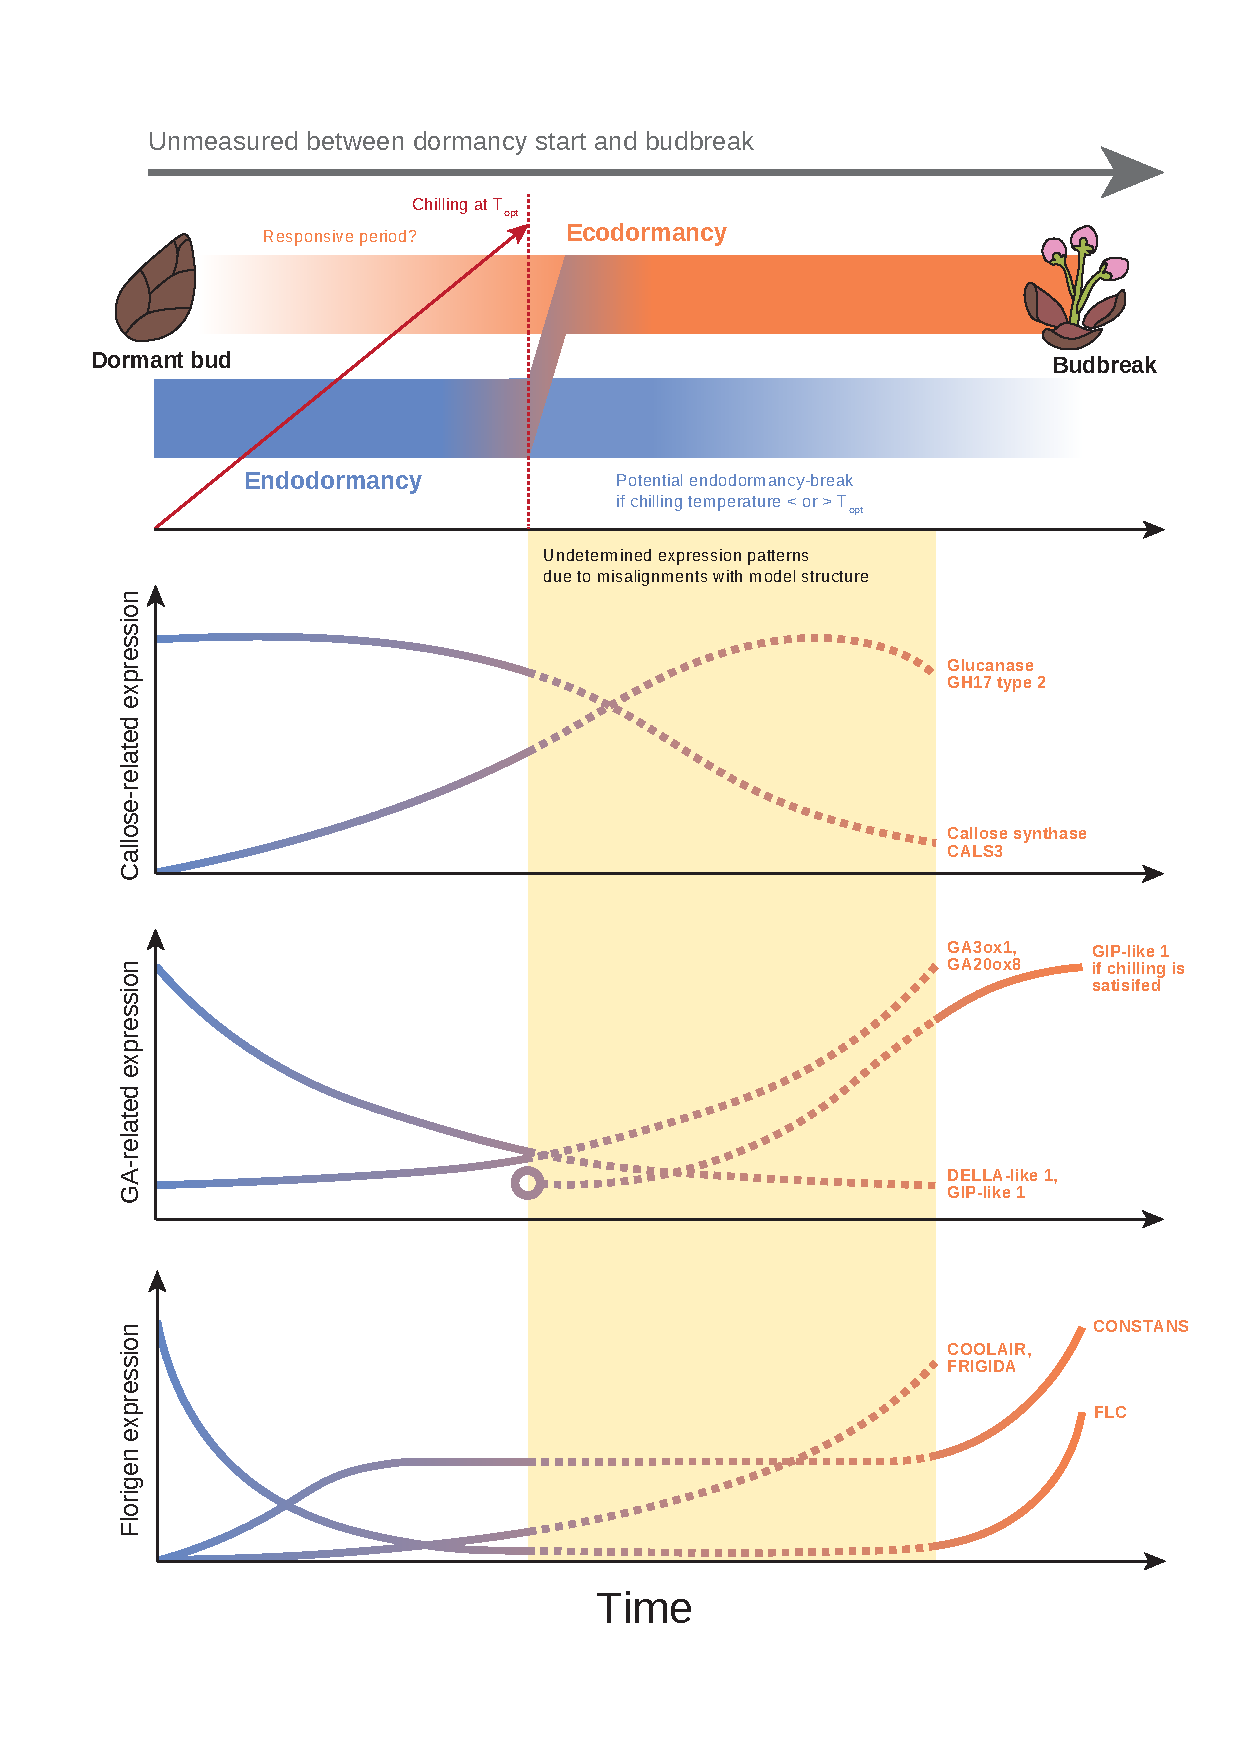
\includegraphics[width=0.7\textwidth]{..//..//figures/conceptModel/conceptModel_gradient.pdf}
\caption{Aligning phenological models and molecular findings. Current phenological models of budbreak (top panel) assume two underlying states that lead to the observed process of budbreak: (1) endodormancy during which plants accumulate sufficient chilling to break endodormancy and transition to (2) ecodormancy, a period during which plants accumulate sufficient `forcing' (warm temperatures) to break bud (flower or leaf). Over 30 variants of this model exist, including those where the phases are sequential (darker shading) or occur in parallel (dark and light shading). Molecular work suggests callose (second panel), alongside gibberellic acid (GA, third panel) and circadian clock-related genes (fourth panel) may all underlie these hypothesized phases.} 
\label{fig:modelsketch}
\end{figure}

\begin{figure}[h!]
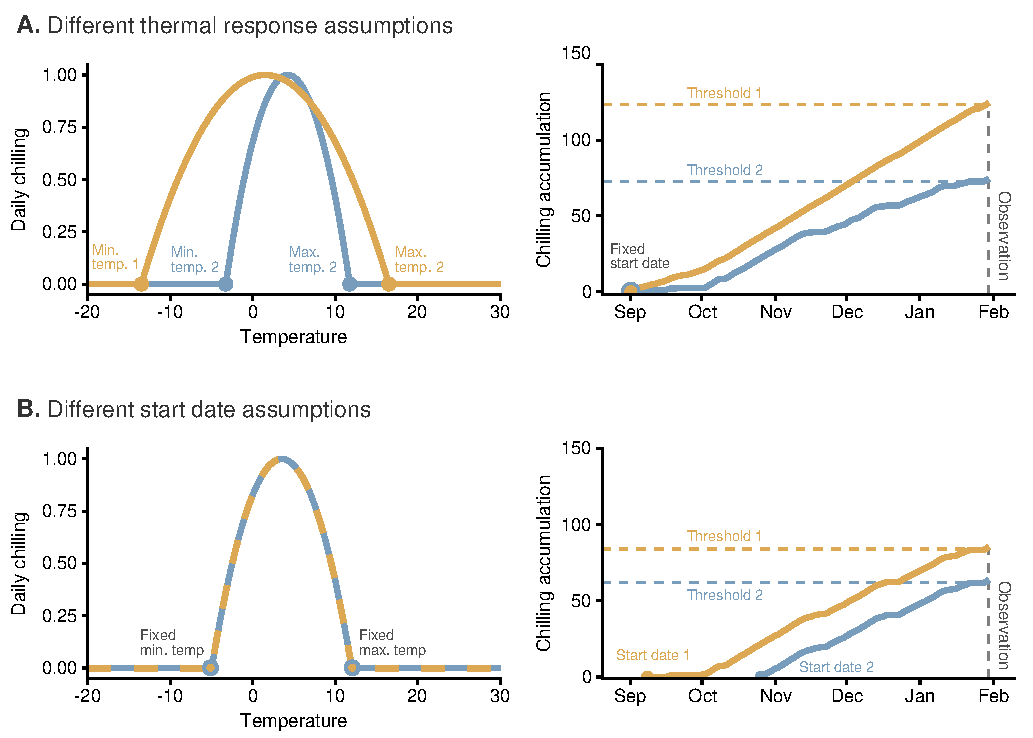
\includegraphics[width=0.8\textwidth]{..//..//analyses/figures/non_identifiability.pdf}
\caption{\textbf{Current models of chilling cannot uniquely estimate the most important aspects of chilling.} We illustrate this using a simple chilling model with a symmetrical thermal response curve, assuming the end of the chilling phase (often called endodormancy break) is observed (dashed vertical lines in right panes). In both cases, multiple parameter sets reproduce the same observation equally well. \textbf{(A)} Estimating the thermal response curve parameters (min. and max. temperatures) and the chilling threshold jointly (with a fixed start date) leads to many potential solutions. For example, a wider temperature range requires a higher threshold to reach the observed date (yellow), while a narrower range requires a lower threshold (blue). \textbf{(B)} The same issue happens when the response curve is fixed but the start date and threshold are estimated jointly. An earlier start date with a higher threshold (orange) leads to the same observed date as a later start date with a lower threshold (blue). 
These two simple examples illustrate that the parameter space contains multiple indistinguishable solutions, even when the end of the chilling phase is known (which is rare, more often models are built with only data on the end of the next phase---observed via budbreak). This issue would be even worse if the thermal response curve, the threshold, and the start date were all estimated jointly---and when the end of the phase is not directly observed. This reality is present in every model of chilling, but rarely discussed and often not even mentioned.} % https://github.com/lizzieinvancouver/chillingconcepts/issues/12} 
\label{fig:nonidentifyme}
\end{figure}




\renewcommand{\refname}{\CHead{}}
\bibliographystyle{/Users/Lizzie/Documents/EndnoteRelated/Bibtex/styles/besjournals}
\bibliography{..//..//refs/bibforchillingconceptms}\end{document}

\end{document}

% \signature{Elizabeth M Wolkovich}
\address{Forest and Conservation Sciences\\
University of British Columbia\\
2424 Main Mall\\
Vancouver, BC V6T 1Z4}


 increasing interest in chilling and new molecular work has led impressive advances, yielding several recent reviews, but none have directly challenged the concept of chilling. 

Our concept piece 



... 

Something about how lots of articles have reviewed chilling and talked about new mechanisms ours is unique in highlighting fundemental problems with the concept that may limit the potential for rapid progress. We ask "Is the concept of `chilling' necessary for scientific progress?"

Current models of chilling predict wildly different leafout times for the same study system and temperature regime \citep{guy2014,chuine2016}. 
Even simple models yield radically different predictions depending on the choice of parameterization

This approach of assigning some unknown parameters as known has the benefit of avoiding adding more unknown model parameters, but has led researchers to be overly confident in a model of chilling where more is actually unobserved and unknown than acknowledged. 

If callose is a major controller of endodormancy and its release, chilling models could be limited to those that match the idea of callose degradation---meaning models that include a temperature range over which the enzyme(s) degrading callose is active (Figure \ref{fig:modelsketch}).

Focused on how chilling can accelerate observable events, researchers have calculated `chilling' required for leafout of forest trees from cutting experiments similar to those used for peaches \citep[reviewed in][]{ospreebbms}, ground observations of budburst \citep{Luedeling2009}, and satellite measures of greenup \citep{kaduk2011predicting}. These estimates rely on phenological models that have become critical across a suite of fields, from climatology, where modeling how vegetation on the land surface responds to anthropogenic climate change affects carbon storage, to crop biology, where `chill units'  guide growers in which specific cultivar to plant and has led to the cross-disciplinary field of phenology \citep{Schwartz:1994he,Cleland:2007or,pmp}. 

\vspace{1.5ex}\\
Please consider our manuscript, ``A simple explanation for declining temperature sensitivity with warming,'' for consideration as a Brief Communication for \emph{Nature Climate Change}. 
\vspace{1.5ex}\\
Climate change has shifted many biological events \citep{IPCC:2014sm}, and recent observations that species sensitivity to temperature is declining have raised concerns that fundamental biological processes are now also changing. Studies suggest warming has altered the main drivers of leafout in temperate plants \citep{fu2015,gusewell2017,Samplonius:2018aa} and altered carbon uptake in the tundra due to increased light limitation or shifts in photosynthesis \citep{piao2017,Zhu2019}. The potential for such ecosystem effects is alarming, but they are rarely reported with strong evidence beyond declines in temperature sensitivity.
\vspace{1.5ex}\\
Here we show that current observations of declining sensitivities---used as evidence of fundamental shifts in underlying biological processes---are an illusion. We combine simple theory and simulations with data from plant development experiments and long-term records to show that declining sensitivities are the null expectation from current methods. This is because many biological events are the outcome of threshold processes and thus will occur more quickly with warming. This in turn will lead to lower estimated responses per degree C when using linear models, without any changes in the underlying biology. When using simple non-linear methods, we find no evidence of declining sensitivities across several empirical datasets \citep[including using the same dataset used in][]{fu2015} . % Effectively, warming acts to step on the biological accelerator, making the use of classic calendar time problematic. % They are instead the outcome of the current methods used to calculate temperature sensitivity with warming.
\vspace{1.5ex}\\
We believe this confusion in interpreting observed declining sensitivities is currently rampant throughout the phenological \citep[e.g.,][]{fu2015,Samplonius:2018aa,meng2020} and related literature \citep[e.g.,][]{piao2017} and may apply more broadly to many fields using linear methods and fixed time periods with warming. Our understanding of this problem only came through close cross-disciplinary collaboration between biologists (Wolkovich group) and statisticians (J. Auerbach and A. Gelman). 
\vspace{1.5ex}\\
%We have suggested several potential reviewers through the online submission site (Julio Betancourt, Theresa Crimmins, Alison Donnelly,  Jarrod Hadfield). 
Based on the manuscript's cross-disciplinary nature, we have suggested reviewers with biological (David Inouye, Theresa Crimmins and Toby Ault) and statistical (Richard McElreath and Jarrod Hadfield) backgrounds. Prior to submission Jonathan Davies, Yongshuo Fu, David Lipson, Christy Rollinson and Yann Vitasse reviewed the manuscript. This manuscript is not under consideration elsewhere. All authors approved of this version for submission. Empirical data are already publicly available through several major data portals, and we provide a link in the main text to our simulation code. % The top three references in this area are Fu \emph{et al.} 2015 (\emph{Nature}), Piao \emph{et al.} 2017 (\emph{Nature Climate Change}) and Meng \emph{et al.} 2020 (\emph{PNAS}).\\
